\subsection{Rabi-Oszillationen}
Die aufgenommene Amplitude des Antwortsignals (Envelope-Signal) als auch das In-Phase Antwortsignal werden gegen die Zeit aufgetragen (siehe Abbildung \ref{fig:rabi}). An die Amplitude des Antwortsignals wird die Funktion
\begin{align*}
  U(t)=U_b+U_o|\sin(\omega t+\delta)|
\end{align*}
angepasst. An das In-Phase Signal wird die Funktion
\begin{align*}
  U(t)=U_b+U_o\sin(\omega t+\delta)
\end{align*}
angepasst. Die jeweiligen Parameter sind in Tabelle \ref{tab:rabi} zu sehen. Bis auf zwei Datenpunkte des Envelope-Signals wird der Verlauf gut von den Regressionskurven beschrieben. An den ermittelten Werten für $\omega$ und $\delta$ ist auch zu erkennen, dass die Signale, wie erwartet, Phasengleich sind. Die unterschiedlichen Werte für $U_0$ kommen durch die im Gerät passierende Umrechnung von Envelope Signal in In-Phase Signal zustande.

\begin{figure}[h]
  \centering
  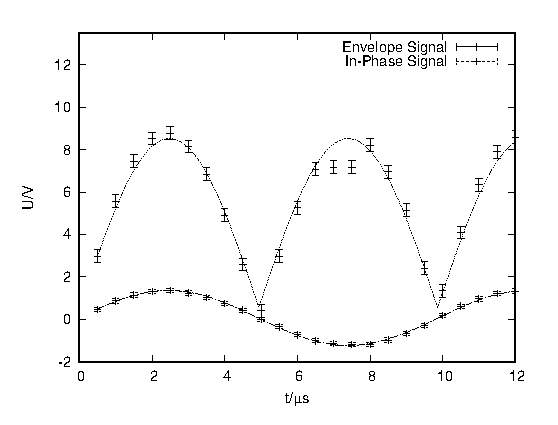
\includegraphics[width=0.75 \linewidth]{data/p402_443_data/rabi_f_1/rabi_1.eps}
  \caption{Rabi-Oszillationen mit Regressionskurven}
  \label{fig:rabi}
\end{figure}

\begin{table}[h]
  \centering
  \begin{tabular}{c c c c c}
    \toprule
    Signal & $U_b/\mathrm{V}$ & $U_0/\mathrm{V}$ & $\omega \cdot \mu\mathrm{s}$ & $\delta$ \\
    \midrule
    Amplitude & $0,6 \pm 0,3$ & $8 \pm 0,3$ & $0,638 \pm 0,005$ & $-0,01 \pm 0,04$ \\
    In-Phase & $0,061 \pm 0,009$ & $1,3 \pm 0,01$& $0,635 \pm 0,003$ & $0,01 \pm 0,02$ \\
    \bottomrule
  \end{tabular}
  \caption{Regressionsparameter für Rabi-Oszillationen}
  \label{tab:rabi}
\end{table}

